\documentclass[twocolumn]{article}
\usepackage[utf8]{inputenc}

\title{Beautiful Empathy\\
\textit{now with Artificial Intelligence and Blockchain}}
%\date{December 2020}
\author{Dario Garcia - dariogarcia@gmail.com}

% \usepackage{natbib}
\usepackage{graphicx}
\usepackage{amsmath}
\newcommand{\lvl}[1]{\vspace{0.5cm}\Large{\textbf{#1}}\vspace{0.2cm}}
\newcommand{\sublvl}[1]{\vspace{0.3cm}\large{\textit{#1}}\vspace{0.1cm}}

\usepackage[margin=0.7in]{geometry}

\usepackage{setspace}
\renewcommand{\baselinestretch}{1.4} 

\begin{document}

\maketitle

\lvl{}
\vspace{-1cm}
\center{\textbf{Beautiful Empathy} is a collaborative app/board/computer game in which players collaborate to create a unique and colorful mosaic.}

\center{The game has no scoring system and there is no official winner.\\ The main outcome of the game is the mosaic built together.}



\begin{figure}[h!]
\centering
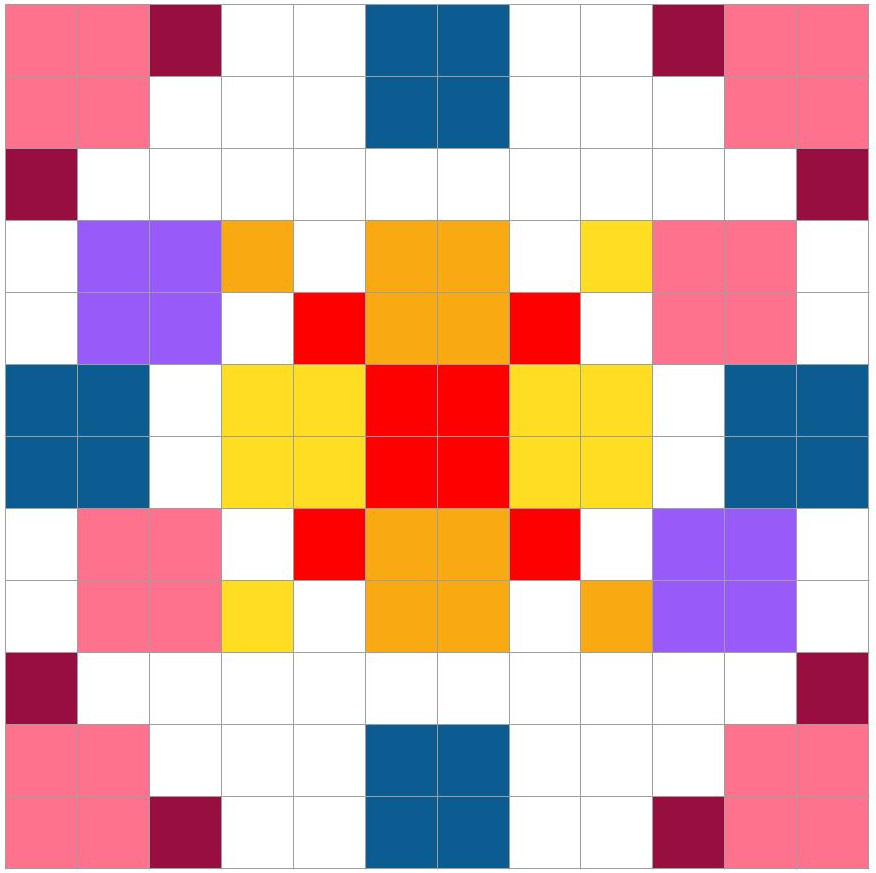
\includegraphics[scale=0.22]{First_ever.jpg}
\caption{Mosaic created with an early version of the game, using a now deprecated color map.}
\label{fig:mosaic}
\end{figure}


\null
\vspace{1cm}
\lvl{The Story}

Lita loves art. She is happy when surrounded by beauty. For her house, Lita wants a unique mosaic, a completely original piece. For that, she hires her favourite artists (you) to paint a shared mosaic in turns.

But before a painting session, Lita likes to spends some time with the painters, trying to understand them. When Lita guesses the painter's minds in these little chats, the artist becomes extra motivated, and is capable of doing more artwork. 

By the end, all that matters is that the painters and Lita, are happy with the resulting artpiece.

\newpage

\begin{figure}[t!]
\centering
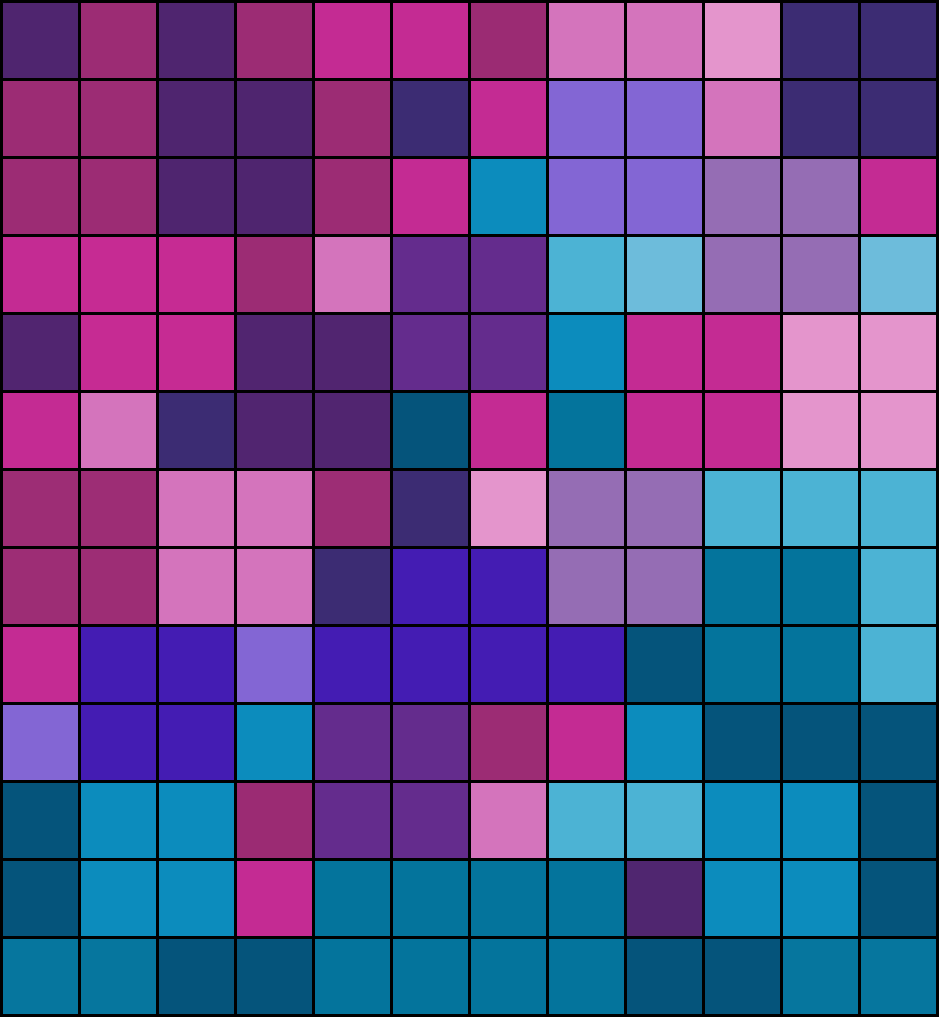
\includegraphics[scale=0.2]{sario210222.png}
\caption{Mosaic created with the circle color map.}
\label{fig:mosaic_2}
\end{figure}


\lvl{Game Script}

The game is played in turns. On each turn, one player is the painter, who will \textit{feel} words in sentences and paint on the mosaic. Another player is Lita, who tries to guess the painter's mind. Typically, roles will rotate among players. Well-intentioned alterations on who plays Lita are welcome. 

\lvl{The Empathy}

Lita tries to figure out which word did the painter choose to complete a sentence, out of two options.

\begin{centering}
\texttt{Sentence:}\\
\textit{The tree was [\ \ \ \ \ \ ] in the middle of the forest}\\
\texttt{Options:}\\
\textit{shaking} | \textit{shinning}\\
\end{centering}
\vspace{0.5cm}

The painter must first read the sentence outloud with the two options, and quickly decide by instinct (and in silence) which one feels better, more fitting. Lita must then guess which of the two options the painter chose. Empathy is key in this part.

At the end of 5 rounds of guesses, count the correct ones. The empathy can be simulated by a uniform random (``Only Beauty'' option).

\lvl{The Beauty}

In this order, the painter:
\begin{itemize}
 \item tries to \textit{add a new color} to it's palette
 \item draws cards to \textit{see the shapes available}
 \item \textit{place the tiles} on the mosaic
\end{itemize}


\sublvl{Add a New Color}

Each player starts the game with one random color. To see if you get a new color, apply the following rules in order until one applies. Consider $C$ is the number of colors owned by the painter, and $G$ the number of correct guesses by Lita. 

\begin{enumerate}
 \item $C<4$ : Get a new color.
 \item $G=5$ : Get a new color.
 \item $G=0$ : Do not get a new color.
 \item $C<G+4$ : Get a new color. 
\end{enumerate}
For example, a painter who owns 5 colors will get a new color if 2 or more questions were correctly answered by Lita. Five correct answers will always get the painter a new color, regardless of the colors already owned.


\begin{figure}[b!]
\centering
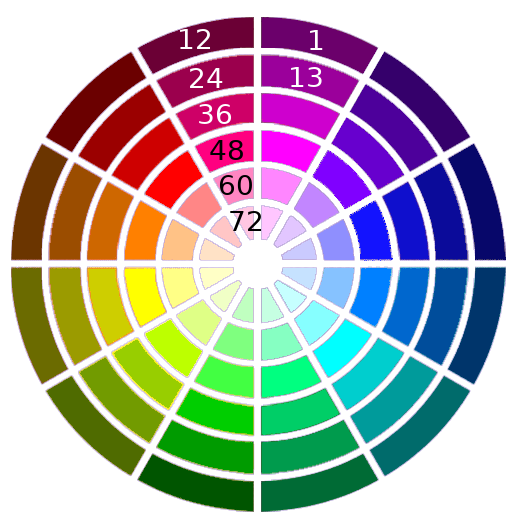
\includegraphics[scale=0.65]{map_1_numbered.png}
\caption{Circle72 Color map. 72 colors, Numbered clock-wise, outside to inside, starting on the pink wedge. Each color is connected with the four colors that surround it. Inner and outer border colors are also connected to all other inner and outer border colors respectively.}
\label{fig:color_map}
\end{figure}

When adding a new color, the painter can choose any color directly connected to a color already owned. The colors each player owns are marked in the color map. A given color can only be owned by a single painter.


\sublvl{See Available Shapes}

After trying to get a color, the painter will find the material it has to work on the mosaic. This will depend on the palette and Litas empathy. A larger palette requires more paint, and more correct guesses motivate the painter further. In detail: 

{\setstretch{1.0}


\begin{itemize}
    \item \textbf{Palette size 1 to 3}:
    \begin{itemize}
        \item If Lita guesses 0 or 1, \\paint for 2 small squares (1x1)
        \item If Lita guesses 2 or 3, \\paint for 4 small squares (1x1)
        \item If Lita guesses 4 or 5, \\paint for 6 small squares (1x1)
    \end{itemize}
    \item \textbf{Palette size 4 to 6}
    \begin{itemize}
        \item If Lita guesses 0 or 1, \\paint for 8 small squares (1x1)
        \item If Lita guesses 2 or 3, \\paint for 4 small squares (1x1) \\and 2 big squares (2x2)
        \item If Lita guesses 4 or 5, \\paint for 8 small squares (1x1) \\and 2 big squares (2x2)
    \end{itemize}
    \item \textbf{Palette size 7 or more}
    \begin{itemize}
        \item If Lita guesses 0 or 1, \\paint for 4 small squares (1x1) \\and 2 big squares (2x2)
        \item If Lita guesses 2 or 3, \\paint for 8 small squares (1x1) \\and 2 big squares (2x2)
        \item If Lita guesses 4 or 5, \\paint for 16 small squares (1x1)
    \end{itemize}
\end{itemize}

}


\begin{figure}[b!]
\centering
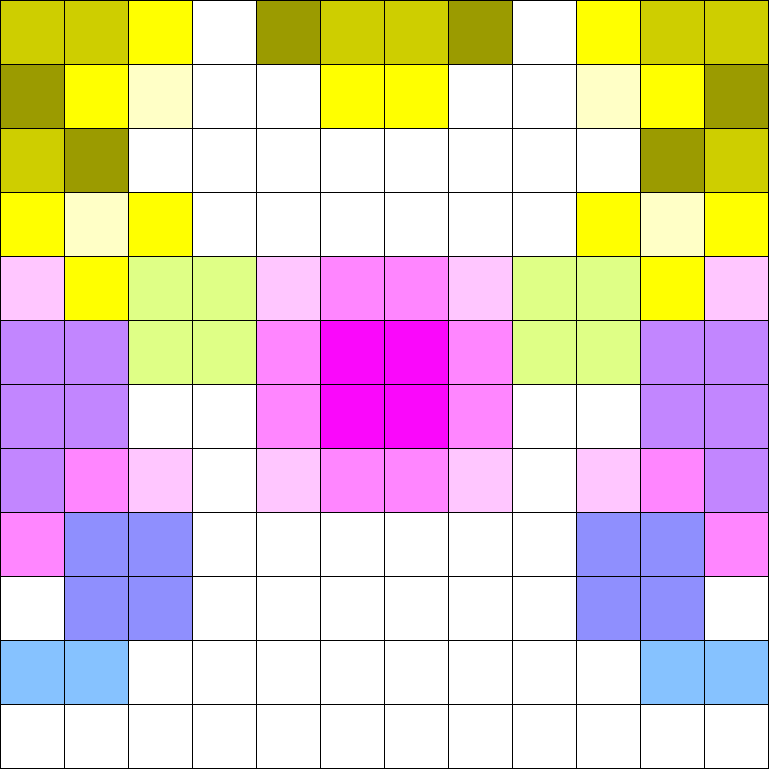
\includegraphics[scale=0.25]{last_mosaic_sario.png}
\caption{Mosaic created with Beautiful Empathy with the Circle71 color map.}
\label{fig:mosaic}
\end{figure}


\sublvl{Place the Tiles}

All that is left to do is for the painter to place the tiles on the mosaic. The painter has absolute freedom to do so, while the other painters can comment on the artistic aspects of it, before and after it is done. The placed tiles can be of any color available in the painter's pallette, and in any combination (different tiles, different colors). Respect for the restrictions of big squares and the work of others, is highly encouraged but not enforced.
% 
% \sublvl{Inspiration Bonus}
% 
% If Lita got 5 correct answers, the painter gains a bonus action, moved by her empathy. The painter draws from a uniform distribution of:
% \begin{itemize}
%     \item Choose and gift any color from the board to a fellow painter. 
%     \item Place 8 tiles on the mosaic with any colors of your choice (owned or not).
%     \item Change the color of 4 tiles already on the board to any of your choice (owned or not).
% \end{itemize}
% 
% 

At this point, this painter's turn is over. Call the next one in!




\lvl{End of Game}

The Game ends after six rounds. Or whenever you want. Once this is happens, take a look at the mosaic you created through empathy, and enjoy the beauty of your collaborative creation.



\lvl{But wait...}

The Artificial Intelligence, right... Well, turns out sentences used to motivate empathy in the game are generated by an AI. We use neural network based language models to generate random but coherent sentences. Then we use the same model to come up with pairs of words which make the same sense in a position within the sentence. This way, when a player picks one word over the other, is out of subjectivity. If the player does so quickly, it becomes a soul-bounding subconscious response.

... and the blockchain ... guess you could turn your mosaics into NFTs or something? :)
% \bibliographystyle{plain}
% \bibliography{references}
\end{document}
